\subsubsection{Зависимость доли уникальных узлов от количества шагов}

В прошлом разделе мы рассматривали доли узлов в виде функций как от количества шагов блуждания $N$, так и от кол-ва уникальных узлов $\Nun = N * \la \nun \ra$, то есть для $n_1 -- n_4$ существует по две лог-лог-шкалируемые функкции функции: $f_i(N)$ \ref{eq:n_i_log_log} и $g_i(\Nun)$ \ref{eq:n_i_u_log_log}

В то же время, была рассмотрена зависимость уникальных узлов $\nun$ от $N$, вследствие чего возникает вопрос взаимозаменяемости этих величин: если $\nun = f_u(N)$, то:

\[ \forall i \in \{1,2,3,4\} \la n_i \ra = g_i(\Nun) = g_i(N * \nun(N))  =? f_i(N) \]

Существования сложной функции в данной зависимости очевидно, но этот момент покажет правильность наших расчётов фитирующих функций, как численно, так и с точки зрения характера шкалирования.
В данном разделе мы рассмотрим графики трёх функций на каждую долю $n_1 -- n_4$: как функцию $f_i(N)$, как функцию $g_i(N*\nun(N))$, а так же аппроксимацию второй функции с целью привести её к виду $f_i(N)$ \ref{eq:n_i_log_log}.
Проведём оценку функции $g_i(N*\nun(N))$ при $N \to \infty$ - коэффициенты фитирующей функции $\nun(N)$ отметим как $k_u, a_u, b_u$, а самой функции $g_i(\Nun)$ - $k_i, a_i, b_i$.

\begin{large}
\begin{equation*}
\begin{array}{l}
\la n_i \ra (\Nun) = k_i * (1/\Nun)^{a_i} + b_i \\
\Nun = N \nun(N) = N (k_u (1/N)^{a_u} + b_u) \\
\end{array}
\end{equation*}	
\end{large}

Проведём линеаризаццию в два шага - сначала $1/\Nun$, а затем $(1/\Nun)^{a_i}$:

\begin{large}
\begin{equation*}
\begin{array}{l}
1) (N (b_u + k_u(1/N)^{a_i})^{-1} = ( N b_u)^{-1} (1 + \frac{k_u}{b_u} (\frac{1}{N})^{a_u})^{-1} = \frac{1}{b_u N} (1 - \frac{k_u}{b_u} (\frac{1}{N})^{a_u} + O(\left(\frac{1}{N})^{2a_u})\right) \\

2) ( - // - )^{a_i}  = (\frac{1}{b_u N})^{a_i} * (1 - \frac{k_u}{b_u} (\frac{1}{N})^{a_u} + O(\left(\frac{1}{N}\right)^{2a_u}))^{a_i} =  (\frac{1}{b_u N})^{a_i} * (1 - \frac{k_u a_i}{b_u} (\frac{1}{N})^{a_u} + O(\left(\frac{1}{N}\right)^{2a_u}))
\end{array}
\end{equation*}
\end{large}

Итоговое выражение примет следующий вид:

\begin{large}
\begin{equation}
\la n_i \ra (\Nun(N)) = \frac{k_i}{b_u^{a_i}} (\frac{1}{N})^{a_i} - \frac{k_i a_i k_u}{b_u^{a_i+1}} (\frac{1}{N})^{a_u+a_i} + b_i + O((\frac{1}{N})^{2 a_u +a_i}),\ \ \ \ \ N \to \infty
\end{equation}
\label{g_n_expect}
\end{large}

Графики изображены на рисунке \ref{fig:ni_fn_vs_gNun}. По ним видно, что функция $f(N)$ и $g(\Nun(N))$ почти не имеют отличий, что говорит о полном взаимозаменяемости аргументов и правильности полученных результатов. Зелёная линия соответствует аппроксимирующему виду $g(\Nun(N))$ и имеет уменьшающуюся при стремлении N к бесконечности поправку, но так же сливается с первыми двумя функциями.

\begin{figure}
\centering
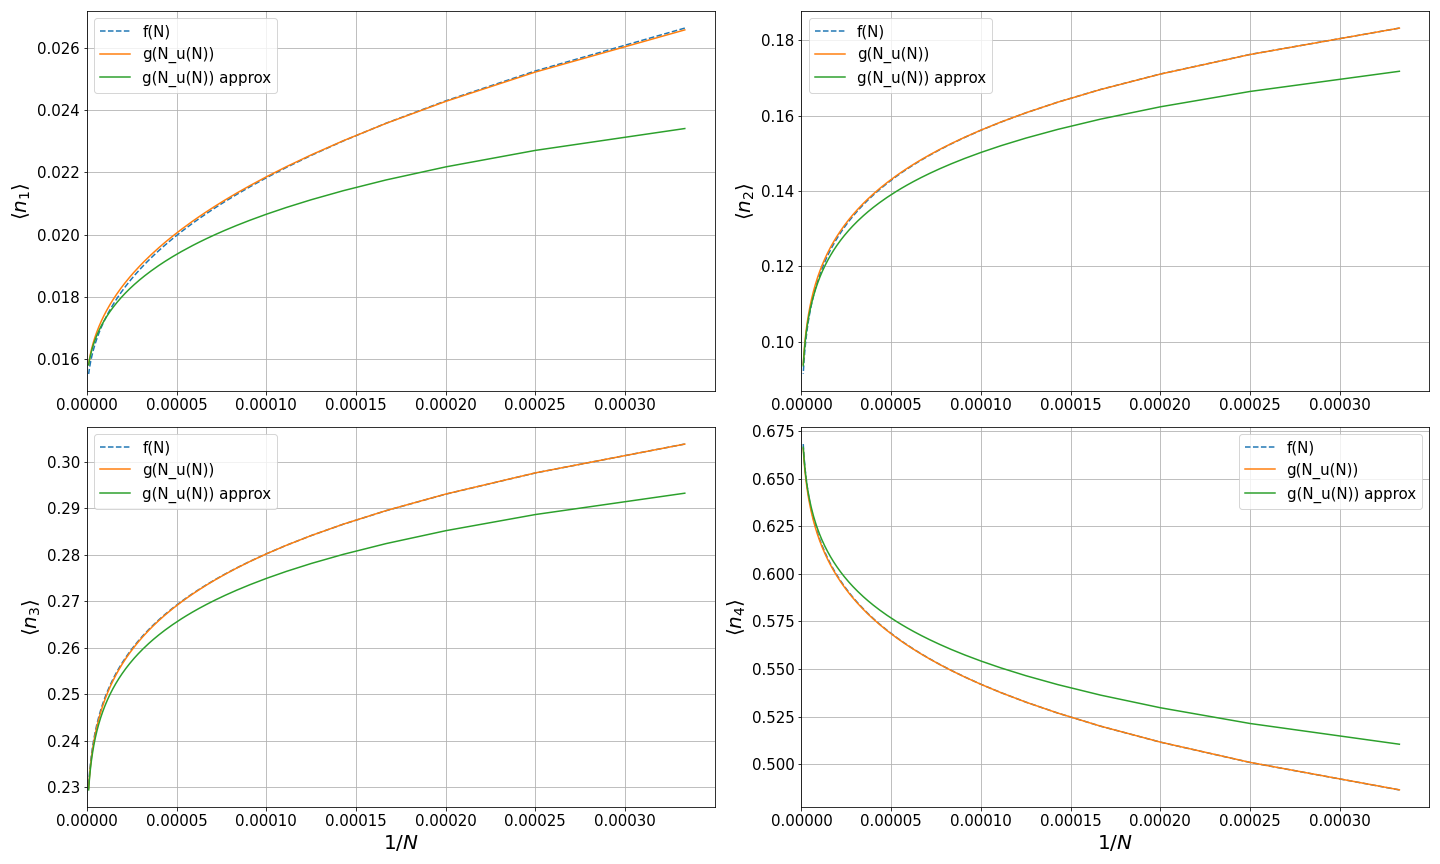
\includegraphics[width=\textwidth]{Sections/Images_2/n_i_fN_vs_gNun.png}
\label{fig:ni_fn_vs_gNun}
\caption{Доли узлов $n_1-n_4$ как функции от количества шагов (синий пунктир), а так же сложные функции от количества уникальных узлов от количества шагов (оранжевая линия - прямая подстановка функций, зелёная - аппроксимация), по горизонтали - обратное количество шагов блуждания 1/N. Функции взяты \ref{eq:n_i_log_log} \ref{eq:n_i_u_log_log} по коэффициетам из таблиц \ref{tab:n_i_log_log} \ref{tab:n_i_u_log_log}}
\end{figure}
